\documentclass[a4paper]{report}

%====================== PACKAGES ======================

\usepackage[french]{babel}
\usepackage[utf8]{inputenc}
%Utilisation de Lorem Ipsum Dolor pour remplir les trous
\usepackage{lipsum}
%pour gérer les positionnement d'images
\usepackage{float}
\usepackage{amsmath}
\usepackage{graphicx}
\usepackage[colorinlistoftodos]{todonotes}
\usepackage{url}
%pour les informations sur un document compilé en PDF et les liens externes / internes
\usepackage{hyperref}
%pour la mise en page des tableaux
\usepackage{array}
\usepackage{tabularx}
%pour utiliser \floatbarrier
%\usepackage{placeins}
%\usepackage{floatrow}
%espacement entre les lignes
\usepackage{setspace}
%modifier la mise en page de l'abstract
\usepackage{abstract}
%police et mise en page (marges) du document
\usepackage[T1]{fontenc}
\usepackage[top=2cm, bottom=2cm, left=2cm, right=2cm]{geometry}
%Pour les galerie d'images
\usepackage{subfig}
%Pour les zones de code
\usepackage{verbatimbox}%simple texte pas coloré
\usepackage{listings}%code coloré (Java ici)
\usepackage{color}

\definecolor{javared}{rgb}{0.6,0,0} % for strings
\definecolor{javagreen}{rgb}{0.25,0.5,0.35} % comments
\definecolor{javapurple}{rgb}{0.5,0,0.35} % keywords
\definecolor{javadocblue}{rgb}{0.25,0.35,0.75} % javadoc
\lstset{language=Java,
basicstyle=\ttfamily,
keywordstyle=\color{javapurple}\bfseries,
stringstyle=\color{javared},
commentstyle=\color{javagreen},
morecomment=[s][\color{javadocblue}]{/**}{*/},
numbers=left,
numberstyle=\tiny\color{black},
stepnumber=2,
numbersep=10pt,
tabsize=4,
showspaces=false,
showstringspaces=false}

\newenvironment*{thanks_perso}{%
\renewcommand*{\abstractname}{Remerciements}
\begin{abstract}
}{\end{abstract}}

%====================== INFORMATION ET REGLES ======================

%rajouter les numérotation pour les \paragraphe et \subparagraphe
\setcounter{secnumdepth}{4}
\setcounter{tocdepth}{4}

\hypersetup{							% Information sur le document
pdfauthor = {Alexandre Kervadec,
		Thibaut Fabre,
		Guillaume Verdugo,
    		Jeremy Arrestier},			% Auteurs
pdftitle = {Projet de Programmation -
			Synchronisation audio-video pour expériences de perception},			% Titre du document
pdfsubject = {Mémoire de Projet},		% Sujet
pdfkeywords = {JavaFX, SQLite, NetBeans, VLCj, Xuggler, CSS, Prosodie, Design, Ergonomie},	% Mots-clefs
pdfstartview={FitH}}					% ajuste la page à la largueur de l'écran
%pdfcreator = {Kile},% Logiciel qui a crée le document

%======================== DEBUT DU DOCUMENT ========================

\begin{document}

%régler l'espacement entre les lignes
\newcommand{\HRule}{\rule{\linewidth}{0.5mm}}

%page de garde
\begin{titlepage}
\begin{center}

% Upper part of the page. The '~' is needed because only works if a paragraph has started.

\includegraphics[width=0.35\textwidth]{./logo}~\\[1cm]

\textsc{\LARGE Master 1 Informatique}\\[1.5cm]

\textsc{\Large }\\[0.5cm]

% Title
\HRule \\[0.4cm]

{\huge \bfseries Projet de Programmation\\
Synchronisation audio-video pour expériences de perception \\[0.4cm] }

\HRule \\[1.5cm]

% Author and supervisor
\begin{minipage}{0.4\textwidth}
\begin{flushleft} \large
\emph{Auteurs:}\\
\textsc{Alexandre Kervadec}\\
\textsc{Thibaut Fabre}\\
\textsc{Guillaume Verdugo}\\
\textsc{Jeremy Arrestier}
\end{flushleft}
\end{minipage}
\begin{minipage}{0.4\textwidth}
\begin{flushright} \large
\emph{Client:} \\
Jean-Luc \textsc{Rouas}\\
\emph{Chargé de TD:} \\
Jeremy \textsc{Frey}
\end{flushright}
\end{minipage}

\vfill

% Bottom of the page
{\large \today}

\end{center}
\end{titlepage}

%page blanche
\newpage
~
%ne pas numéroter cette page
\thispagestyle{empty}
\newpage

\begin{thanks_perso}
Nous tenons tout particulièrement à remercier Jeremy Frey, notre chargé de TD, qui a toujours été de bons conseils et qui nous a permis d’avancer lorsque nous étions en difficulté.
% Nous tenons aussi à adresser nos remerciements à Jean-Luc Rouas qui nous a offert l’opportunité de participer à son projet, et ainsi mettre nos connaissances au service de la recherche.

Pour finir, nous remercions M. Narbel pour ses cours et ses conseils qui ont été le fil conducteur de notre projet.
\end{thanks_perso}

%page blanche
\newpage
~
%ne pas numéroter cette page
\thispagestyle{empty}
\newpage

\renewcommand{\abstractnamefont}{\normalfont\Large\bfseries}
%\renewcommand{\abstracttextfont}{\normalfont\Huge}

\begin{abstract}
\hskip7mm

\begin{spacing}{1.3}
 
 
En étant en contact avec des personnes venant  de l’université Bordeaux Montaigne et de l’université de Waseda à Tokyo, ce projet nous permet de comprendre la prosodie selon certaines langues qui sont déjà définies dans un corpus créé par des chercheurs (français, japonais, anglais américain et portugais du brésil) pour des situations prédéfinies. 

Ce projet vise à étudier la façon dont  un utilisateur peut construire un document audio-vidéo à partir d’un son (exprimant par exemple l’admiration) et d’une vidéo (exprimant par exemple le mépris) exprimant par exemple l’ironie. L’utilisateur peut être amené à utiliser les données enregistrées dans sa langue natale ou non, dans le but d’étudier les correspondances entre les langues. 

Notre but est donc de réaliser une interface graphique permettant de réaliser des tests prosodiques\footnote{Prosodie : ``La prosodie (ou la prosodologie) est une branche de la linguistique consacrée à la description (aspect phonétique) et à la représentation formelle (aspect phonologique) des éléments de l’expression orale tels que les accents, les tons, l’intonation et la quantité, dont la manifestation concrète dans la production de la parole, est associée aux variations de la fréquence fondamentale (F0), de la durée et de l’intensité (paramètres prosodiques physiques). Ces variations étant perçues par l’auditeur comme des changements de hauteur (ou de mélodie), de longueur et de sonie (paramètres prosodiques subjectifs)''.\cite{di2000} } sur des cobayes.
L’administrateur peut lister, ajouter ou supprimer du contenu dans la base de données du test pour pouvoir s’il le souhaite mettre à jour celle-ci. Les utilisateurs auront quant à eux à inscrire des informations personnelles pour participer aux tests et auront par la suite le choix entre deux modes. Soit il peut choisir un mode entrainement pour se familiariser avec le logiciel soit effectuer le vrai test. Dans ces deux modes, les utilisateurs auront à faire un choix d’une vidéo parmi plusieurs, à fusionner avec une bande son parmi une autre liste.
Ce mix de vidéo/son devra donner une réponse à une question du type : “Réaliser une vidéo qui exprime l’ironie.” A la fin de chaque test les données utilisateurs et les réponses aux questions seront extraites pour pouvoir faire des statistiques.

\end{spacing}
\end{abstract}


\tableofcontents
\thispagestyle{empty}
\setcounter{page}{0}
%ne pas numéroter le sommaire

\newpage

%espacement entre les lignes d'un tableau
\renewcommand{\arraystretch}{1.5}

%====================== INCLUSION DES PARTIES ======================

~
\thispagestyle{empty}
%recommencer la numérotation des pages à "1"
\setcounter{page}{0}
\newpage

\chapter{Analyse de l'existant}

\section{Compréhension du sujet}\label{comprehension_sujet}

La prosodie est un terme complexe mettant en exergue les liens entre les expressions (faciales et vocales) et les émotions qui en découlent. Néanmoins, nous ne pouvons réduire cette définition à ce simple résumé, de ce fait l'article \cite{bachorowski1999vocal} nous permet d'obtenir une définition plus précise sur ce terme technique.

Ainsi, la voix est un élément important de la prosodie car elle est un acteur primordial de la transmission d'émotions mais en fonction de nos origines socio-culturelles cette perception peut différer \cite{auberge2002prosodie}.
De plus, la voix se combine avec les expressions faciales qui sont le portrait de l'émotion que nous voulons transmettre. Les changements que nous effectuons sur notre visage(position des sourcils, lèvres...) permettent l'expression d'émotions par celui-ci \cite{ekman2003unmasking} .

Enfin, le document \cite{fourer:hal-00992083} nous offre une approche sociétale du problème avec une étude sur la prosodie attitudinale concernant la langue japonaise.


\section{Références sur la transformation de la voix}\label{ref_transfo_voix}

Pour les études prosodiques, des modulations, des découpages et des modifications en tous genres de la voix sont nécessaires mais cette dernière est un mécanisme complexe comme cela nous est présenté dans le cours de Ricardo Gutierrez-Osuna \cite{Gutierrez-Osuna:ISP-PMS} et l'article de l'IEEE Signal Processing Letters \cite{haagen1994transformation}.

L'extrait de la IEEE International Conference on Acoustics de 1998 \cite{Acero:ICASSP98-II-881} décrit deux possibles modifications prosodiques.

La méthode Gestalt est une méthode de psychothérapie qui s'appuie sur la manière dont les personnes entrent en contact, se comportent dans une relation. C'est une methode qui peut s'appliquer à notre projet \cite{auberge2002gestalt}.

Coupler PSOLA (Pitch Synchronous Overlap and Add) qui est une technique de traitement de signal permettant d'effectuer des traitements sur les discours à un module pour les transformations spectrales peut nous permettre de créer un système de conversion de voix \cite{valbret1992voice}.

\section{Références sur l'expression faciale}\label{ref_transfo_faciales}

Par rapport à un discours précis, les expressions faciales, et particulièrement buccales, peuvent être régies par plusieurs règles de synchronisation afin de pouvoir, par exemple, améliorer un discours homme-machine \cite{beskow1995rule} .

La prosodie faciale permet, en outre, d'aider à la détection ethnique du protagoniste, qui est un facteur intéressant pour notre projet car il porte sur quatre langues : le français, l'anglais (américain), le portugais du Brésil et le japonais\cite{matsumoto1992american}.


\section{État de l'art}\label{state_of_the_art}

La prosodie permet, par exemple, d'aider à la reconnaissance des différents dialectes arabes. En d'autres termes, malgré une proximité géographique et linguistique, la prosodie permet la différenciation\cite{rouas2006identification}.

L'apprentissage de la prosodie n'est pas un désir extrêmement nouveau. Ainsi nous nous sommes documentés sur l'état actuel de l'art en matière de logiciel concernant l'apprentissage de la prosodie et nous avons trouvé certains documents proches de ce que l'on désirait développer \cite{10.4000/alsic.332}. 

\section{Programmation avec du contenu vidéo}

Une vidéo ne se réduit pas seulement à un format, elle se compose aussi des \textit{Codecs}. Ces dispositifs permettent la compression/decompression d'un signal numérique. Ces \textit{Codecs} sont des mécanismes importants lorsque l'on veut faire du traitement sur une vidéo. C'est effectivement cette technique qui permet l'encodage et le décodage de fichier afin de pouvoir les lire \cite{ghanbari1999video} \cite{he2013introduction}.
\section{Ergonomie}
Pour designer notre application, nous devons suivre des règles et des principes existants afin de mêler harmonieusement ergonomie et design \cite{lente2014scenariser}.

\section{Base de données}

Durant ce projet, il a fallu trouver le système de base de données le plus adapté à nos besoins. Pour ce faire, nous nous sommes appuyés sur l'article \cite{strauchnosql}, disséquant l'architecture \textit{NoSQL} (Not Only SQL).
Nous nous sommes finalement tournés vers le \textit{SGBDR} (Système de Gestion de Base de Données Relationnelles) \textit{SQLite} et nous sommes informés sur l'utilisation et les finalités de ce logiciel \cite{kreibich2010using}.


 
\chapter{Analyse des besoins}

\section{Fonctionnement de l'application}

Nous exposons d'abord le fonctionnement global de l'application, c'est à dire tous les états dans lesquels il sera possible de se trouver, comment y arriver et comment en sortir.

 \begin{figure}[!ht]
 \begin{center}
  \fbox{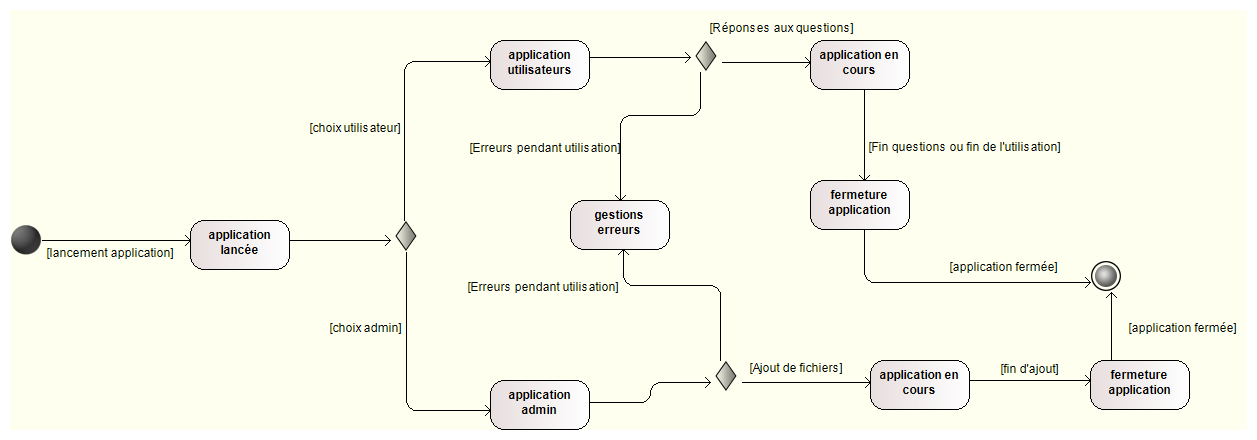
\includegraphics[width=17cm]{besoins/etattrans.png}}
  \caption{Diagramme d'états - Fonctionnement de l'application}
  \label{etattrans}
 \end{center}
 \end{figure}


\section{Classement par priorité des besoins}\label{priorite}

Les besoins sont classés par priorité dans leur ordre d'apparition. De plus, chaque besoin se voit attribué un niveau de priorité comme suit :

\begin{itemize}
 \item[-] Priorité critique
 \item[-] Priorité moyenne
 \item[-] Priorité basse
 \item[-] Facultatif
\end{itemize}

\section{Besoins fonctionnels}\label{besoins_fonctionnels}

\subsection{Utiliser l’application sur les systèmes d’exploitation principaux et récents}\label{systems}

\subsubsection{Description}

Etant donné que notre client sera amené à transporter l’application, il faut que celle-ci puisse fonctionner sur différents environnements à savoir \textit{Microsoft Windows 7}, \textit{Ubuntu 12.04}, \textit{Debian 6.0}, \textit{MAC OS X 10.9} et les versions plus récentes de ces systèmes d’exploitation.
L’application est susceptible de fonctionner sur d’autres systèmes d’exploitation (par compatibilité de noyau) sans toutefois de garantie de ce fonctionnement.

\subsubsection{Faisabilité}

Cette condition est remplie en utilisant une application \textit{JavaFX}, supportée par les environnements possédant un environnement \textit{Java} à jour (la version 8 étant nécessaire pour le fonctionnement optimal de \textit{JavaFX}).

\subsubsection{Contingence}

Le risque principal serait que le client travaille sur une machine ne possédant pas un environnement \textit{Java} à jour. Pour pallier ce problème, nous proposerons un script d'installation du dernier environnement \textit{Java}.

\subsubsection{Test}

Lancer l'application dans chacun des systèmes d’exploitation cités précédemment. L'application devra fonctionner sur chacun d'entre eux, sans quoi, la contrainte ne serait pas remplie.

\subsubsection{Priorité : \textit{Critique}}

\subsection{Rendre l'application nomade}\label{nomadite}

\subsubsection{Description}

Pour effectuer ses études, notre client ne souhaite pas transporter sa machine sur les lieux où elles se déroulent. Pour cela, il faut donc avoir une application transportable sur un périphérique externe de type clef USB.

\subsubsection{Faisabilité}

Pour remplir cette condition, tous les composants de l’application compilée seront stockés sur une clef USB ou un disque dur externe, afin que le client puisse l'utiliser sur n’importe quel ordinateur.

\subsubsection{Contingence}

Le risque serait que le formatage de la partition de la clef USB ne soit pas pris en compte par le système d’exploitation de la machine (par exemple le formatage \textit{NTFS} de \textit{Windows} est reconnu par le système \textit{Mac OS}, mais accessible en lecture seule, le formatage \textit{EXT4} du système \textit{Ubuntu} n’est pas reconnu par les systèmes d’exploitation \textit{Windows}). Pour éviter cela, la clef devra être formatée en \textit{FAT32}, qui est un formatage de partition reconnu par les systèmes d’exploitation cités dans la section \ref{systems}.

\subsubsection{Test}

Faire fonctionner l’application à partir d’une clef USB (ou disque dur externe selon le support qui sera choisi) sur les différents systèmes d’exploitation cités précédemment. L'application devra fonctionner en \textit{standalone}, sauf dans le cas d'un environnement \textit{Java} non à jour, comme précisé en \ref{systems}.

\subsubsection{Priorité : \textit{Critique}}

\subsection{Ajouter du contenu multimédia et des questions}

\subsubsection{Description}

Le client doit pouvoir enregistrer dans la base de données, de nouvelles vidéos et de nouveaux sons afin d'améliorer l’efficience de ses tests. De plus, pour améliorer ses recherches, notre client pourra ajouter des questions avec leurs correspondances audios et vidéos.
Cet ajout de médias devra être possible en ligne de commande sous un système \textit{Unix}, en passant un fichier texte dans un paramètre.

\subsubsection{Faisabilité}

Pour faciliter cette gestion, nous utiliserons une base de données. Les données seront plus facilement accessibles lors de l’utilisation de l’application.
Puis, pour réaliser l'administration en ligne de commande, une application annexe sera développée. Cette application sera en \textit{Java} et disposera des arguments nécessaires pour ajouter et lister les médias dans la base de données.

\subsubsection{Test}

Ajouter du contenu multimédia (audio et video) et une question puis lister tout le contenu de la base de données pour voir si l’ajout à été pris en compte.
Une réussite du test se concluera par une base de données remplie via l'application annexe, et une application graphique qui fonctionnera (qui accèdera au médias et les affichera).

\subsubsection{Priorité : \textit{Moyenne}}

\subsection{Exploiter différents formats de fichiers audio et vidéo}

\subsubsection{Description}

Le contenu multimédia de notre client étant composé de différents formats vidéo et audio, utilisants des codecs variés, l’application doit pouvoir assurer une lecture optimale de ces médias.

Effectivement, c’est un obstacle que l’on rencontre dès que l’on commence à programmer dans le domaine de la vidéo et de l’audio (des références étudiant certaines de ces contraintes : \cite{ghanbari1999video} et \cite{he2013introduction}).
Le fond du problème est l’utilisation de Codecs (vidéo et audio) pour lire les différents types de fichiers, qui sont encodés selon différentes normes.

Les formats que l’on doit pouvoir supporter sont les suivants :\\

%\begin{table} Fait planter le positionnement vertical du tableau.
\begin{center}
\begin{tabular}{c|c}
\textbf{Formats audio} & \textbf{Formats vidéo} \\
\\
\hline
\\
\textit{mpeg2} & \textit{mp4 (H.264)}\\
\textit{aac} & \textit{mov}\\
\textit{wav} & ~
\end{tabular}
\end{center}
%\end{table}
\vspace{0.6cm}

\subsubsection{Faisabilité}

Une solution que nous avons trouvé est le lecteur de médias \textit{VLC Media Player}\footnote{http://www.videolan.org/vlc/}.

Ce lecteur va nous permettre d'utiliser les formats vidéo et audio présentés précédemment. De plus, c'est un logiciel accessible (gratuit et sous licence open-source).

De surcroit, il existe une version portable de \textit{VLC Media Player} permettant un transport optimal sur une clef USB ou un disque dur externe. Cette condition répond à notre besoin de transportabilité évoqué précédemment.

\subsubsection{Contingence}

%Partie a modifier pour le jvlc
Le risque d’utiliser ce genre de logiciel peut être l'impossibilité d'intégrer le lecteur dans une interface graphique \textit{JavaFX} (solution choisie dans la section \ref{systems}). Si cette solution n’est pas possible, on pourra ouvrir un lecteur en \textit{standalone}\footnote{Utilisation de l'application à part entière, et pas dans un plugin ou une extension.}.

\subsubsection{Test}

Création d’un script qui ouvrira toutes les vidéos disponibles et vérifiera si une erreur est survenue.

\subsubsection{Priorité : \textit{Moyenne}}

\subsection{Récupérer les questions et résultats des tests}

\subsubsection{Description}

L’application a pour but de répondre à une série de questions dont les réponses sont une vidéo et un son.\\
Ces combinaisons sont importantes pour notre client, nous devons donc les récupérer.

\subsubsection{Faisabilité}

La solution à ce besoin serait une base de données stockant l’ensemble des questions, sons, vidéos et réponses attendues.
L’application devra ensuite exporter les réponses et l'identité de l'utilisateur sous forme d’un fichier \textit{txt}, fichier qu’exploitera le client.   

\subsubsection{Test}

Demander à faux sujet de mener le test, et vérifier les données exportées dans le fichier \textit{txt}. Il sera possible de lire le contenu de cet export facilement, avec un éditeur de texte.

\subsubsection{Priorité : \textit{Moyenne}}

\subsection{Rassembler des informations sur les sujets}

\subsubsection{Description}

Afin d'exploiter les résultats des tests, le client veut récupérer des informations sur les sujets.
Les informations que l’on doit récupérer sont les suivantes :\\
\begin{itemize}
 \item[-]  nom
 \item[-]  prénom
 \item[-]  sexe
 \item[-]  date de naissance
 \item[-]  langue maternelle
 \item[-]  si la langue maternelle est différente de celle du test, nombre d’année d’études de cette langue
\end{itemize}

\subsubsection{Faisabilité}
  
Pour répondre à ce besoin, il faut implémenter un formulaire au lancement de l’application.

\subsubsection{Test}

Faire essayer l’application à une tierce personne puis vérifier que toutes les informations sur la personne ont bien été récupérées.

\subsubsection{Priorité : \textit{Faible}}

\section{Besoins non-fonctionnels}\label{besoins_non-fonctionnels}

\subsection{Permettre une maintenance du logiciel}

\subsubsection{Description}

L’application que nous allons livrer ne sera pas une finalité mais seulement une étape dans un projet beaucoup plus vaste. Ainsi, d’autres personnes devront probablement modifier cette application afin de répondre à de nouveaux besoins. Ces nouveaux développeurs devront disposer de tous les éléments nécessaires pour comprendre notre travail. 

\subsubsection{Faisabilité}

Il est possible de répondre à ce besoin en documentant notre code. Il existe par exemple en \textit{Java}, la \textit{Javadoc}, qui est générable avec des commentaires spéciaux. Elle est exportable en \textit{HTML} et contient toutes les explications necessaires à la compréhension du code. 

De plus, il faudra ajouter des commentaires quand une fonction sera trop complexe et que des indications intermédiaires seront nécessaires.

\subsubsection{Test}

Demander à un développeur externe au projet d’essayer de comprendre notre code, et d'ajouter une fonctionnalité.

\subsubsection{Priorité : \textit{moyenne}}

\subsection{Bénéficier d’une ergonomie efficiente}

\subsubsection{Description}

L’application sera ergonomique pour permettre au sujet de se concentrer principalement sur le test et pas sur le fonctionnement de ladite application. De plus, le sujet soumis au test sera possiblement novice en informatique, l’application devra ainsi être intuitive.

\subsubsection{Faisabilité}

Pour satisfaire ce besoin, nous devons mettre en place un graphisme épuré de tout accessoires détournant l’attention. De plus, nous utiliserons des couleurs de ton pastel pour éviter de fatiguer le regard de l’utilisateur.

Cette contrainte peut être satisfaite en s’inspirant de nombreux designs qui ont déjà été développés et publiés sur le web. On s’appuiera notamment sur l’article \cite{lente2014scenariser} qui étudie la \textit{“collaboration entre Ergonomie, Design et Ingénierie”}.

\subsubsection{Test}

Utilisation de l’application par plusieurs sujets sans donner d’indication sur son fonctionnement afin d’observer si le design affecte négativement l'expérience de l’utilisateur.

\subsubsection{Priorité : \textit{basse}}

\section{Prototype d'application}

 Un \textbf{\textit{prototype}} de rendu est proposé ci-dessous. L'application finale que nous présenterons pourra diférer quelque peu de ce prototype.

\begin{figure}[!ht]
 \begin{center}
  \fbox{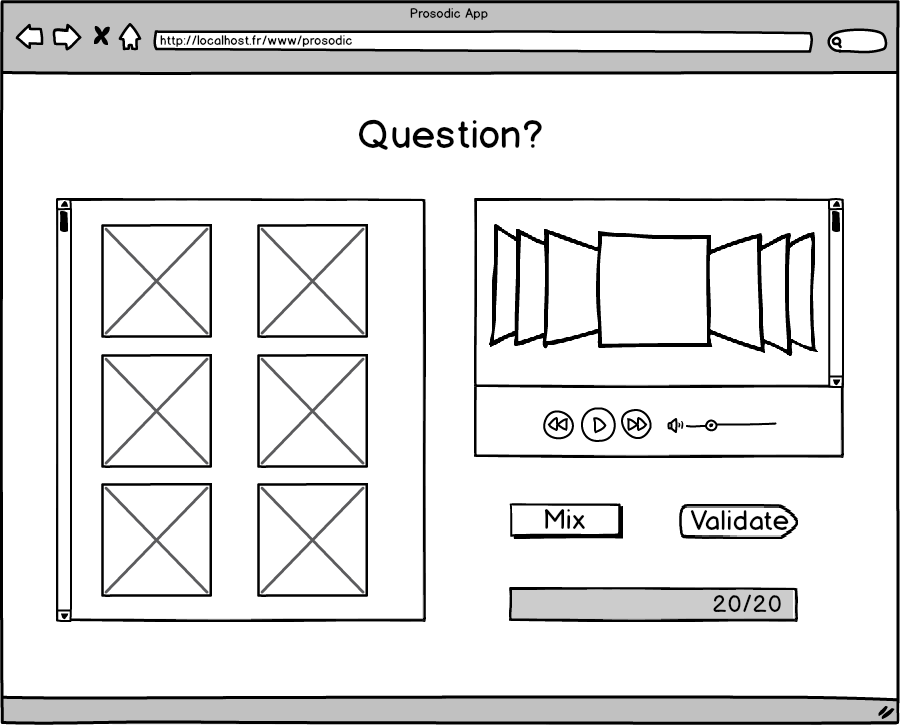
\includegraphics[width=6cm]{besoins/T-3.png}}
  \caption{Prototype d'application}
  \label{prototype}
 \end{center}
 \end{figure}
 
 \section{Gestion du temps}
 
 Afin de mieux organiser notre temps et répartir équitablement le travail, nous avons établi un diagramme de Gantt, détaillant chaque étape de ce projet de programmation.
 
 \begin{figure}[!ht]
 \begin{center}
  \fbox{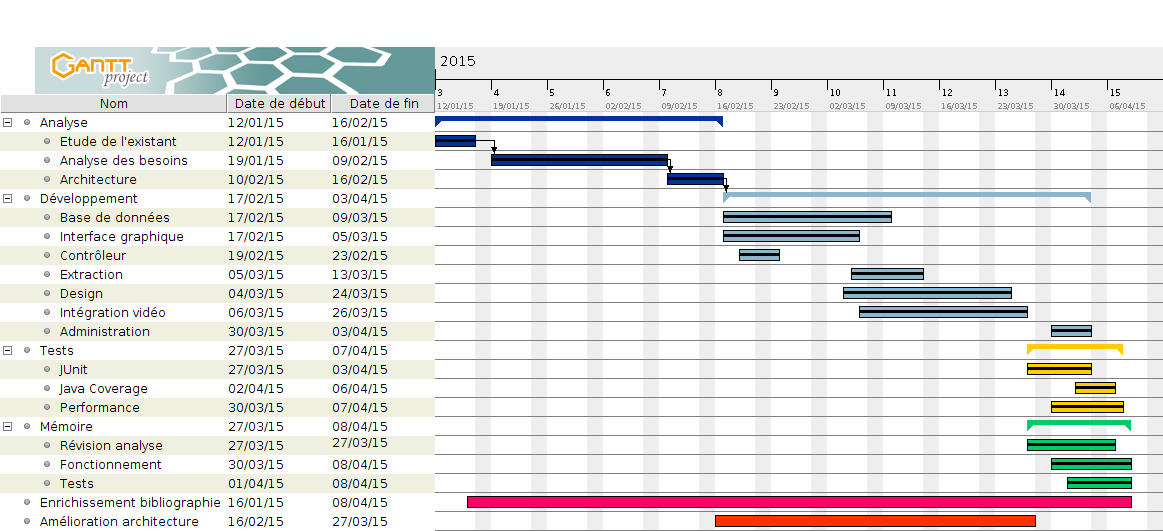
\includegraphics[width=17cm]{besoins/Gantt.png}}
  \caption{Gestion du temps - Diagramme de Gantt}
  \label{Gantt}
 \end{center}
 \end{figure}

\chapter{Architecture}
 
\begin{figure}[!h]
\begin{center}
  \fbox{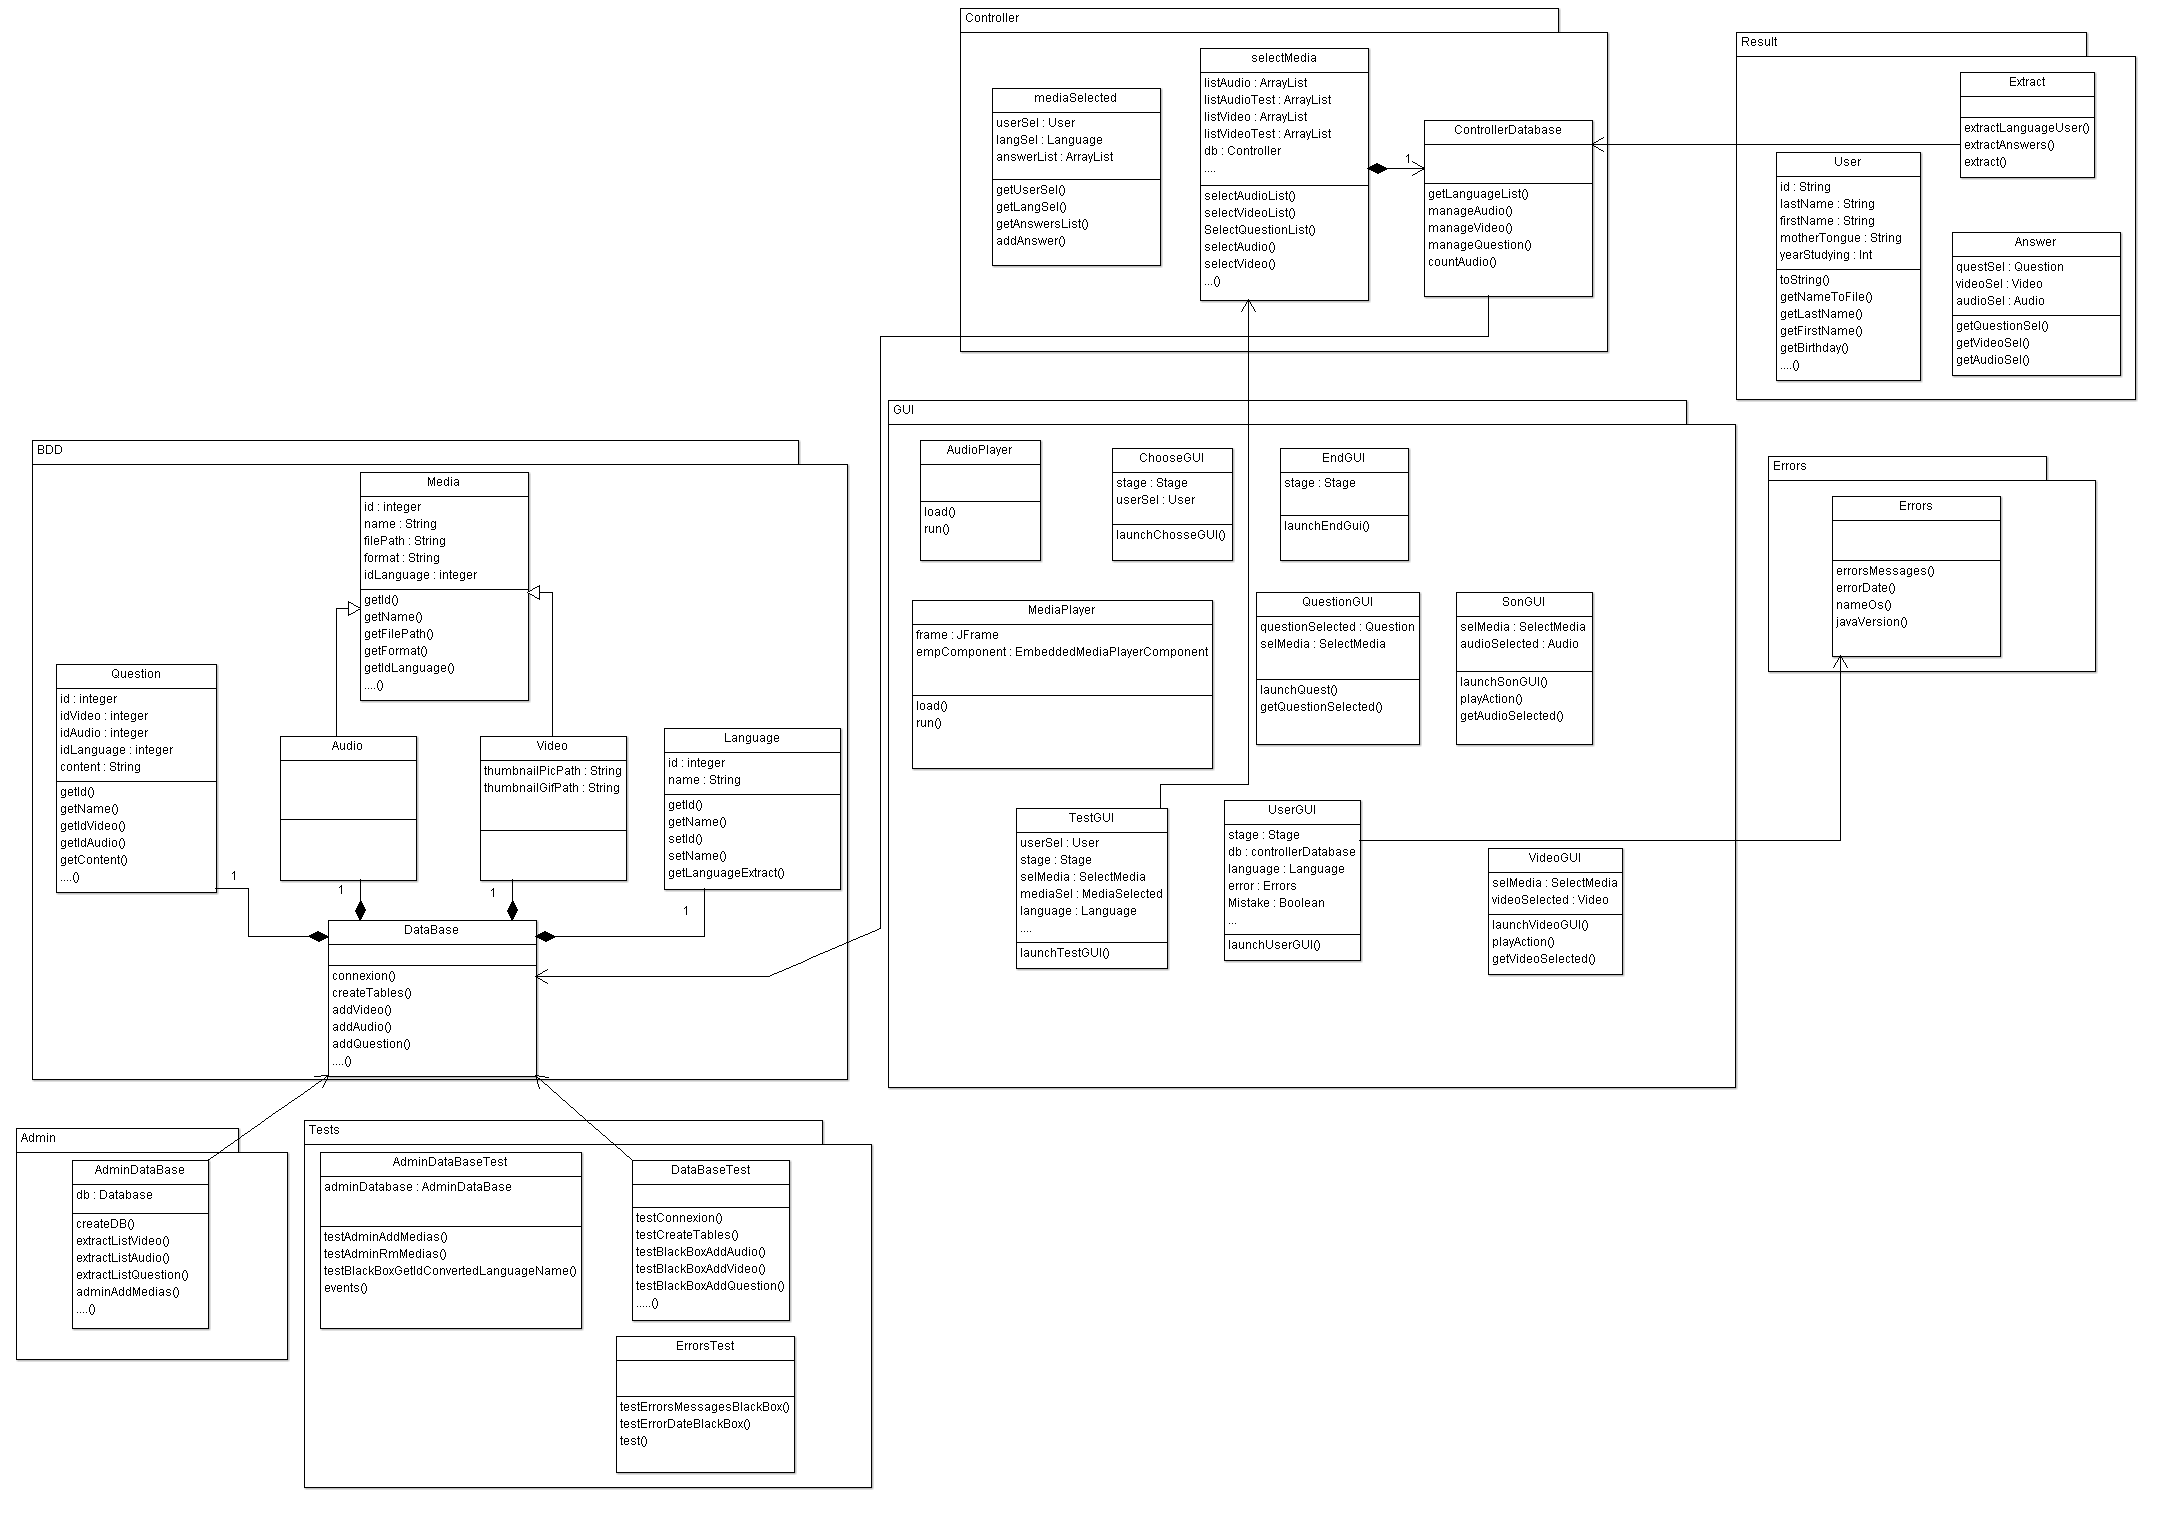
\includegraphics[width=18cm,angle=90]{./architecture/architecture.png}}
  \caption{UML - Architecture}
  \label{diaglog} 
\end{center}
\end{figure}

L'architecture \textbf{M}odele-\textbf{V}ue-\textbf{C}ontroleur (\textbf{MVC}) permettant ``la séparation des éléments principaux d'un système d'intéraction d'une couche présentation''\footnote{Citation du cours magistral de PdP de M.Narbel} nous semblait le pattern le mieux adapté au développement de notre application basée sur les liens base de données/interface graphique. 

De plus, grâce à ce \textit{design pattern}, nous avons pu répartir les rôles de chacun afin de produire un travail efficace.

\section{Explication détaillée des packages}

Notre architecture est structuré en plusieurs packages. Ils ont été créés avec comme but de compartimenter notre architecture en fonction des besoins renseignés précédemment. Chaque package regroupe un certain nombre de classes, chacune possédant une fonction bien précise.

Dans cette section, nous allons décrire le besoin que nous avons voulu satisfaire avec chaque package et le rôle de chacune de leurs classes. Pour suivre la logique MVC, nous allons structurer la description selon ce même pattern.

\subsection{Modèle}


\subsubsection{BDD}

Ce package concerne tout ce qui se rapproche de la base de données. Ainsi, elle possède tous les types d'objets que nous allons insérer et sélectionner :
\begin{itemize}
 \item \textit{Media}
  \subitem \textit{Video}
  \subitem \textit{Audio}
 \item \textit{Language}
 \item \textit{Question}
\end{itemize}


Ces types d'objet intéragissent avec la base de données via la classe \textit{Database}.

Nouvelle langue > simple et rapide.

\paragraph{Classe DataBase}

Cette classe contient toutes les intéractions entre les objets et la base de données (on notera BDD dès à présent). Elle permet de :

\begin{itemize}
 \item se connecter à la BDD (créer et initialiser la BDD le cas échéant)
 \item remplir la BDD
 \item rechercher dans la BDD
 \item supprimer des éléments dans la BDD
 \item consulter la BDD
\end{itemize}


Cette centralisation permet d'optimiser l'accès à la BDD, faciliter la gestion de conlits et gérer les échanges de médias à partir du même endroit.

\paragraph{Classes Media, Audio et Video}

Ces trois classes sont unies : les classes \textit{Audio} et \textit{Video} héritent de la classe abstraite \textit{Media}. Cette dernière regroupe les méthodes communes aux classes héritées. Celles-ci sont importantes dans notre application puisqu'elles créent les objets en fonction du contenu de la base de données. Ils serviront pour la lecture des médias dans notre application grâce aux \textit{file\_path} (chemin vers les fichiers sur le disque) renseignés dans la base données.

\paragraph{Classe Question, Language}

Ces classes créent des objets correspondants à une question et à une langue. Les langues nous permettrons de sélectionner les questions, audios et vidéos qui seront proposés à l'utilisateur de l'application.

Il n'était pas forcemment nécessaire de créer une classe pour la langue, mais nous avons trouvé ceci utile, au cas où notre client souhaite par la suite traiter de nouvelles langues.


\subsection{Contrôleur}


\subsubsection{Controller}

\paragraph{ControllerDatabase}

Cette classe fait le lien entre le modèle et la vue, c'est elle qui récupère les méthodes du modèle, pour les utiliser dans la vue, et inversement. Ses méthodes n'affectent par contre pas directement la vue, car elles sont utilisées par les deux autres classes du packages pour générer des objets de média voulus.

\paragraph{SelectMedia}

Réalise une sélection des médias nécessaires à l'initialisation des pages de la vue.

\paragraph{MediaSelected}

Cette classe permet de récupérer les medias qui ont été sélectionnés par l'utilisateur, afin de pouvoir exporter ces données, via le package \textit{Result} (voir \ref{Archi_Results}).


\subsubsection{Result}\label{Archi_Results}

Ce package a pour fonction de regrouper les classes qui seront utiles pour l'étude de notre client. Il est constitué d'une classe qui rassemble les informations sur l'identité de l'utilisateur, d'une autre qui liste les réponses de celui-ci effectuées lors du test et enfin d'une classe qui extrait toutes ces données dans un fichier.

\paragraph{Classe User}

Cette classe se compose de différents attributs qui permettent de différencier chaque sujet, dans le but futur, de réaliser des statistiques.

\paragraph{Classe Answer}

Cette classe regoupe un trio d'objets composé de \textit{Question}, \textit{Audio} et \textit{Video} qui correspondent à la réponse audio et vidéo pour la question posée à l'utilisateur.

\paragraph{Classe Extract}

Cette classe sert à extraire, dans un fichier, la langue du test, les données de l'utilisateur ainsi que les réponses de celui-ci. Elle n'est composée que de méthodes statiques. En effet, on a trouvé inutile de créer un objet pour cela vu que la méthode principale n'est appelée qu'une unique fois dans l'application. Chaque extraction est effectuée lorsque l'utilisateur valide sa dernière réponse.


\subsection{Vue}


\subsubsection{GUI}

Ce package regroupe toutes les configurations et les fonctionnalités de l'interface graphique.

\paragraph{Classe Start}

C'est à partir de cette classe que l'application se lance.
Cette classe permet de créer et de charger l'environnement commun à toutes les fenêtres de l'interface graphique. C'est à dire :
\begin{itemize}
 \item la taille de la fenêtre
 \item la feuille de style  et la police personnalisée
 \item le titre de la fenêtre
\end{itemize}


\paragraph{Classe UserGUI}

Cette classe correspond à l'interface graphique où l'utilisateur renseigne son identité et choisit la langue du test.

\paragraph{Classe ChooseGUI}

Cette classe permet à l'utilisateur de choisir entre la session d'entrainement et la session test.

\paragraph{Classe TestGUI}

Cette classe est assez spéciale vu que plusieurs objets graphique gravitent autour d'elle. En effet, on peut dire que l'interface qui en résulte est composé de quatre composants : l'audio, la vidéo, les question et les différents boutons pour le mix et la validation. La classe place tous ces objets dans le panel de la scene. 


\subsection{Tests}

Ce package regroupe l'ensemble des tests qui seront necessaires pour minimiser les erreurs au niveau de la base de données (par exemple lors d'un upload de médias, on vérifie que le format soit adapté). Pour être plus précis, il s'agit des tests suivants :
\begin{itemize}
 \item Tests unitaires avec \textit{JUnit}
 \item Tests de performance avec les outils de \textit{Netbeans}
\end{itemize}

\chapter{Fonctionnement et tests}

Dans cette partie nous chercherons à décrire dans un premier temps les fonctionnements, ou, le cas échéant, les non fonctionnements de notre application.  Nous aborderons ensuite la politique de tests effectuée pour vérifier notre code. 

\section{Fonctionnement}

Lorsque l'on lance l'application, on exécute l'interface graphique. Cette interface fait appel aux autres parties de l'architecture pour afficher et organiser ses composants.

\subsection{Interface Graphique (GUI)}\label{GUI}

Tout d'abord, nous allons expliquer notre choix de technologie, qui s'est orienté vers le \textit{JavaFX}.
Nous pensions dans un premier temps développer l'application en \textit{Java} et générer des pages \textit{HTML} pour l'interface graphique. Puis après des recherches, nous avons découvert le \textit{JavaFX}, qui nous permettait de créer une interface graphique, mais à l'instar de la libraire \textit{Swing}, complètement personnalisable. Nous avons alors choisi ce langage afin d'avoir une application 100\% \textit{Java}.


La méthode \textit{main} de Start.java est appelée lors du démarrage de l'application. Cette méthode fait créé une instance de UserGUI, la première page de l'application qui s'affiche.

\begin{figure}[!ht]
\begin{center}
  \fbox{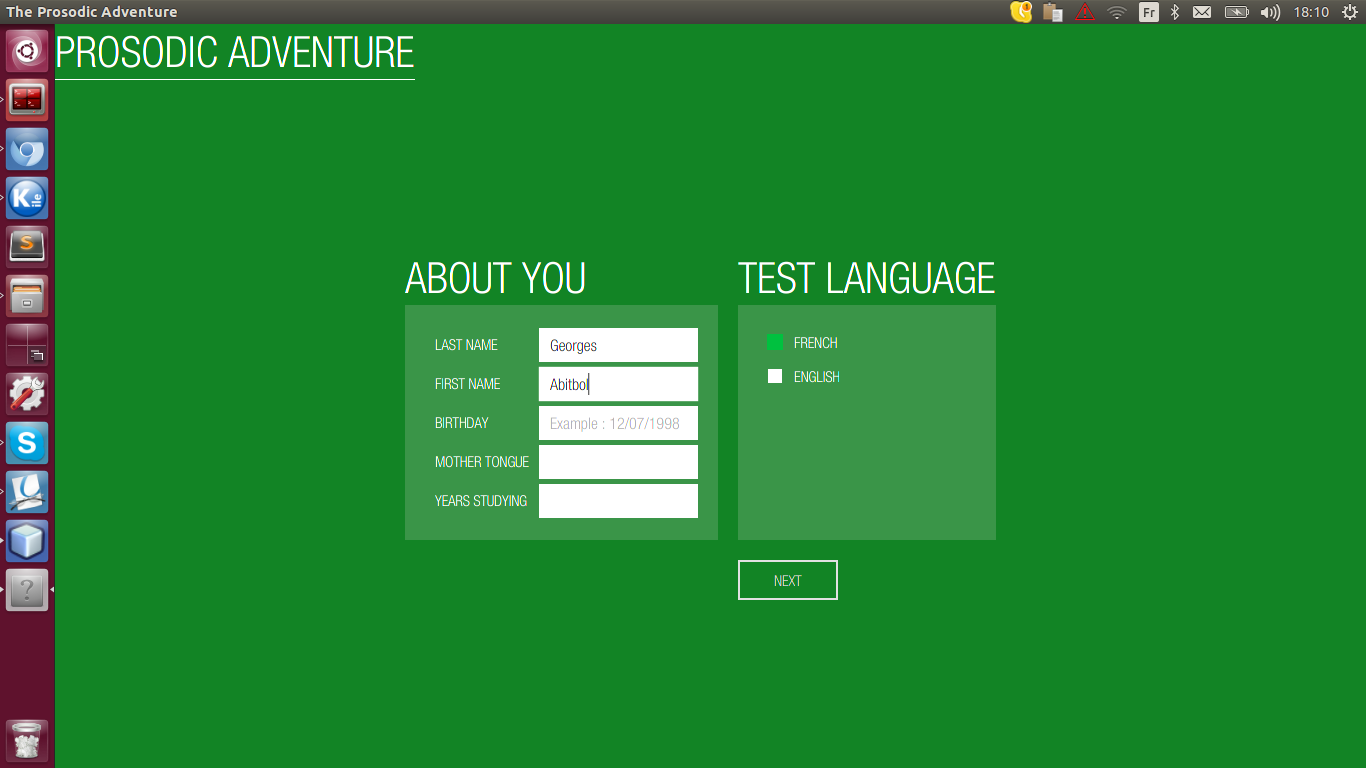
\includegraphics[width=8cm]{./fonctionnement_tests/UserGUI.png}}
  \caption{Fonctionnement - UserGUI}
  \label{UserGUI} 
\end{center}
\end{figure}

Pour récupérer les langues disponibles, UserGUI fait appel au contrôleur, dont nous décrirons le fonctionnement par la suite.
Les informations entrées par l'utilisateur dans les champs de ``\textsc{about you}'' (voir \textsc{Figure} \ref{UserGUI}) sont récupérés lors du clic sur le bouton ``\textsc{next}''. Ces données sont récupérées dans un fichier \textit{txt} par le biais du package \textit{Extract} que nous allons voir plus tard.

Après l'exportation des données sur l'utilisateur, un lien est fait vers la seconde page de l'interface : ChooseGUI (voir \textsc{Figure} \ref{ChooseGUI}). Cette page est une simple page avec deux boutons pour savoir dans quel mode veut aller l'utilisateur (apprentissage da l'application ou test concret).

\newpage

\begin{figure}[!ht]
\begin{center}
  \fbox{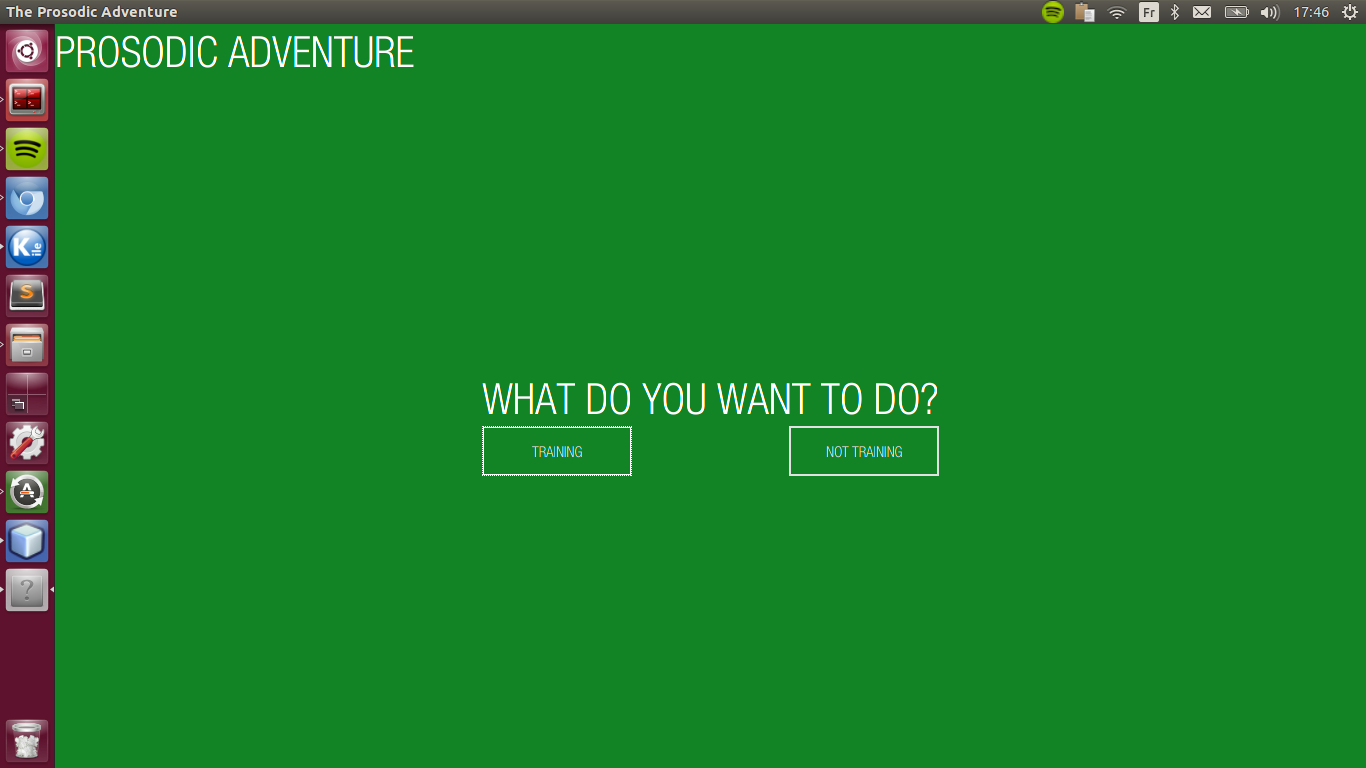
\includegraphics[width=8cm]{./fonctionnement_tests/ChooseGUI.png}}
  \caption{Fonctionnement - ChooseGUI}
  \label{ChooseGUI} 
\end{center}
\end{figure}

On est ensuite dirigé vers le page de test (identique dans le mode ``\textsc{training}'' et ``\textsc{not training}''). La seule différence entre les deux mode est l'exportation de données : dans le test réel, les données sont exportées tandis que dans le mode de découverte, rien n'est exporté.
Les données exportées sont :
\begin{itemize}
 \item Les questions posées
 \item La vidéo réponse
 \item L'audio réponse
\end{itemize}
Ces données sont exportées lors du passage à la question suivante.
Ces précédentes données sont un choix parmis plusieurs. Ces listes de choix sont sélectionnées par les sous-classes \textit{SonGUI}, \textit{VideoGUI} et \textit{QuestionGUI} qui font le lien vers le contrôleur (voir \ref{controller}) afin de récupérer les médias dans la base de données.

\begin{figure}[!ht]
\begin{center}
  \fbox{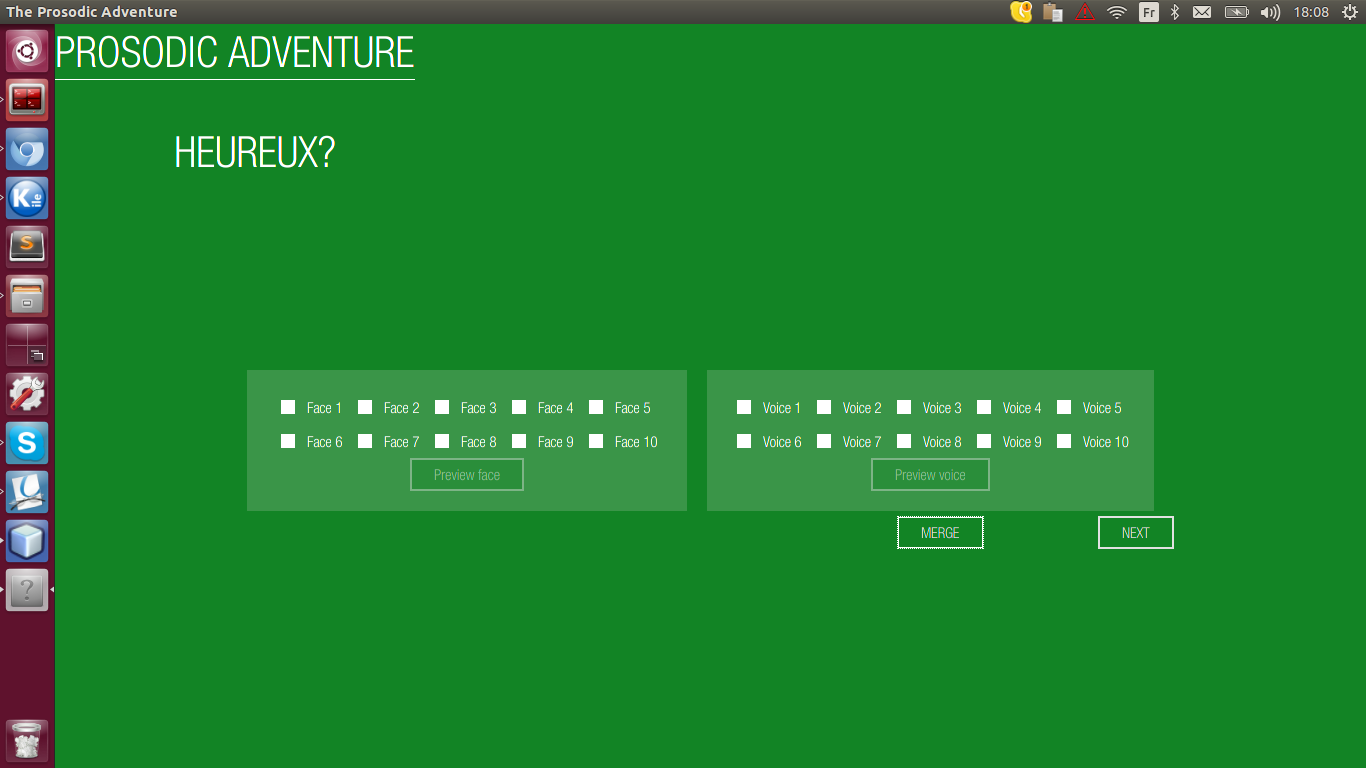
\includegraphics[width=8cm]{./fonctionnement_tests/TestGUI.png}}
  \caption{Fonctionnement - TestGUI}
  \label{TestGUI}
\end{center}
\end{figure}

Les boutons ``\textsc{preview}'' permettent de voir le contenu des vidéos et d'écouter les sons disponibles dans les différentes listes. Afin d'être joués, les médias sont ouverts (voir \textsc{Figure} \ref{VLC} avec VLC (en \textit{standalone}) en faisant appel à la librairie VLC inclue dans le projet (librairie implémentaée dans la classe \textit{MediaPlayer}). Nous avons choisi d'utiliser ce lecteur de médias car le lecteur par défaut de \textit{JavaFX} est trop strict au niveau des codecs vidéo et audio qu'il accepte. VLC, quant à lui, nous offre la possibilité de lire la totalité des médias que l'on doit traiter. Ensuite, la stratégie du \textit{standalone} a été utilisée, car une intégration d'un lecteur non natif \textit{JavaFX} nécessite l'utilisation de la librairie \textit{Swing}, qui connait énormément de problèmes d'intégration à l'interface \textit{JavaFX}.

Ceci reste tout de même une voie intéressante d'amélioration. Nous avons nous même tenté de palier à ce problème, en convertissant les médias à la volée, en utilisant l'extension \textit{Xuggler}. Cependant, ceci demandait beaucoup de temps, et la duplication de tous les médias (ce qui n'est pas négligeable compte tenu de notre besoin d'avoir une application nomade, donc légère).

\begin{figure}[!ht]
\begin{center}
  \fbox{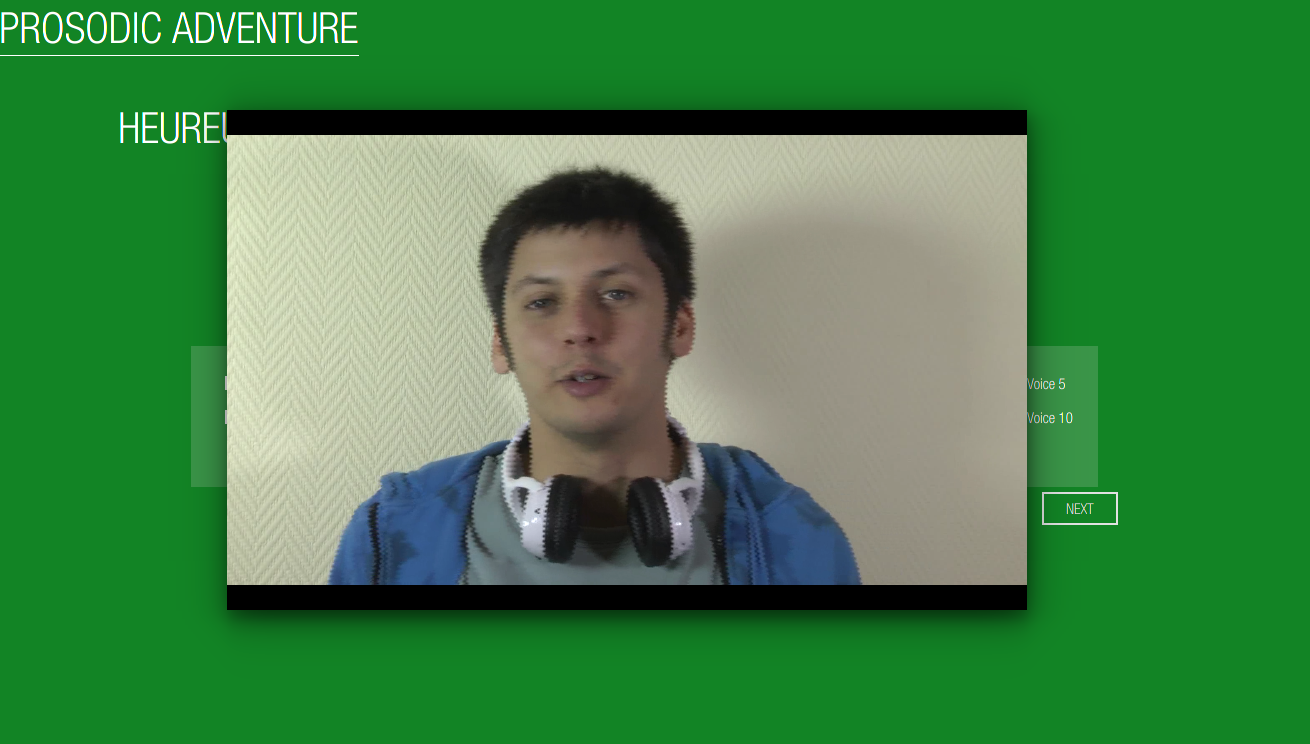
\includegraphics[width=8cm]{./fonctionnement_tests/VLC.png}}
  \caption{Fonctionnement - TestGUI}
  \label{VLC} 
\end{center}
\end{figure}

Finalement, une fois le test terminé, l'utilisateur est redirigé vers une page terminal contenant juste un message de remerciements, ainsi qu'un bouton ramenant vers la première page (\textit{UserGUI}).

\begin{figure}[!ht]
\begin{center}
  \fbox{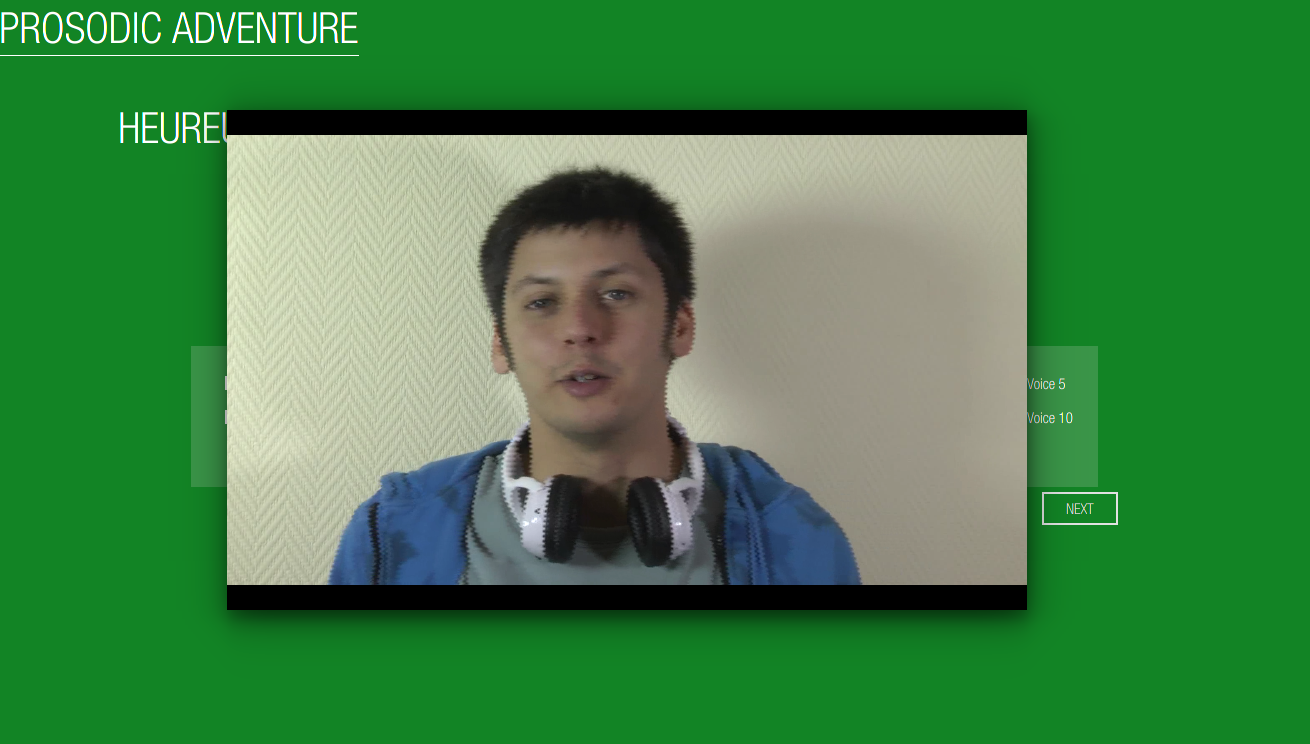
\includegraphics[width=8cm]{./fonctionnement_tests/VLC.png}}
  \caption{Fonctionnement - EndGUI}
  \label{endGUI} 
\end{center}
\end{figure}

\subsection{Base de données}\label{BDD}

Le système de gestion de base de données relationnelles (SGBDR) choisi a été \textit{SQLite}. Ce SGBDR est utilisable sur n'importe quelle plateforme, sans nécessiter l'installation et la mise en place d'un serveur, il se résume à un fichier \textit{.db} qui contient toute la base de données.
Pour le fontionnement de l'application, des méthodes d'accès à la base de données ont été necessaires à implémenter :


\begin{itemize}
 \item Création de la base de données et de ses dépendances (si elle n'existe pas)
 \item Remplissage de la base de données
 \item Consultation du contenu de la base de données
 \item Recherche dans la base de données selon plusieurs critères
 \item Tirage au hasard d'un media de la base de données
 \item Suppression d'un media de la base de données, tout en vérifiant l'intégrité des relations (voir exemple plus en fin du paragraphe suivant)
\end{itemize}


Toutes ces implémentations sont fonctionnelles. Des tests ont été réalisés dessus (voir \ref{tests}).
Les accès à la base de données sont effectués par le driver\footnote{sqlite-jdbc-3.8.7} \textit{Java} de \textit{SQLite}.

Pour éviter tout conflit lors de l'accès à la base de données, des transactions manuelles ont été mises en place : un verrou est créé à chaque accès, ainsi un double accès ne peut pas être effectué.
Etant donné que \textit{SQLite} ne gère pas les contraintes de clef étrangère, nous avons établi un système de vérification en \textit{Java}. Cette vérification vérifie avant chaque modification sensible (suppression d'une vidéo qui pourrait être liée à une question par exemple), qu'aucune dépendance ne sera brisée.


\subsection{Contrôleur}\label{controller}


Le contrôleur étant le lien entre la base de données (modèle) et l'interface graphique (vue), il est appelé à être utilisé à chaque échange entre la vue et le modèle.
Considérant la partie \ref{GUI}, on peut comptabiliser 3 appels :

\begin{itemize}
 \item Lors de l'affichage de UserGUI (\textsc{Figure} \ref{UserGUI}), pour retrouver les languages de test disponibles. L'appel est fait vers une méthode de la classe \textit{ControllerDatabse}, elle-même faisant le lien vers la bonne méthode du package \textit{BDD.DataBase}.
 \item Lors du chargement de la question dans \textit{TestGUI} (\textsc{Figure} \ref{TestGUI}), pour récupérer une question de la base de données, à partir des sous-classes de l'interface graphique citées dans \ref{GUI}. Cette récupération fait appel à la classe \textit{SelectMedia}, elle-même créant une liste de médias retournée par le package \textit{BDD}.
 \item Lors du passage à une question suivante dans l'interface graphique \textit{TestGUI}, car les réponses choisies par l'utilisateur sont récupérées, afin de générer une trace de son test. Ces réponses sont donc récupérées par la classe \textit{MediaSelected}, qui fait cette fois un lien vers le package \textit{Result}, que nous décrirons en \ref{export}.
\end{itemize}


\subsection{Exportation des données}\label{export}

Tout ce qui concerne l'exportation des données se situe dans le package \textit{Result}. Ce package est séparé en 
 éléments :
 
 \begin{itemize}
  \item \textit{Answer.java} qui permet de créer un objet \textit{Answer} afin centraliser les données à extraire.
  \item \textit{User.java} qui a la même fonction que la classe précédente, mais qui contient les informations sur l'utilisateur (informations récupérées dans l'interface \textit{UserGUI}, voir \ref{GUI}).
  \item \textit{Extract} extrait les données contenues dans les deux précédents types d'objet, et les écrit dans un fichier texte, comme dans l'exemple suivant :
 \end{itemize}
 
 \begin{verbnobox}[\small]
  Langage:   French
  User:
      First Name:   Georges
      Last Name:   Abitbol
      Birthday   09/08/1979
      Mother Tongue   French
      Years learning tongue selected   1
  List of answers
      Answer 1:
	    Question:   Pouvez-vous exprimer la douleur avec ces audios et vidéo ?
	    Video   ADMI_B_ok
	    Audio   ADMI

 \end{verbnobox}
 
 
\subsection{Administration}\label{fonction_admi}

L'administration est une application qui fonctionne indépendamment de l'application graphique. Elle est lancée en ligne de commande (\textit{java -jar <fichier.jar> <paramètre 0> <paramètre 1> <paramètre 2>}), les paramètres correspondants aux différentes fonctionnalités. Nous allons décrire le fonctionnement de cette application en partant des choix de paramètres possibles, récapitulés ci-dessous :

\begin{figure}[!ht]
\begin{center}
\begin{tabularx}{17cm}{|c|p{6cm}|X|}
 \hline
 Paramètre 0 & Paramètre 1 & Paramètre 2\\
 \hline
	& video		& \tabularnewline
 add	& audio		& <fichier>\tabularnewline
	& question	& \tabularnewline
\hline
	& video		& \tabularnewline
 rm	& audio		& <fichier>\tabularnewline
	& question	& \tabularnewline
\hline
	& video		& \tabularnewline
 ls	& audio		& \tabularnewline
	& question	& \tabularnewline
 \hline
\end{tabularx}
\end{center}
\caption{Fonctionnement - Utilisation de l'application d'administration}
\end{figure}


\subsubsection{Des paramètres aux actions}

Ce paramètre correspont à quel type d'action on veut effectuer :
\begin{itemize}
 \item add : ajouter du contenu
 \item rm  : supprimer du contenu
 \item ls  : afficher du contenu
\end{itemize}

\paragraph{add}

L'ajout de contenu se fait par le biais d'un fichier (sans extension) contenant du simple texte.
Ce texte doit être formatté selon les règles suivantes :
\begin{itemize}
 \item Ajout de vidéos : le nom d'une vidéo par ligne, selon la syntaxe :
  \begin{verbnobox}[\small][0-9]*\_[0-9]*\_[0-9]*\_[a-zA-Z0-9]*\_[a-z]{2}\_[a-zA-Z0-9]*\_[a-zA-Z0-9]*.[a-zA-Z0-9]*\end{verbnobox}
  Comme par exemple :
 \begin{verbnobox}[\small]
  2013_3_20_S33_fr_L1_OBVI_B_ok.mp4
  2013_3_20_S33_fr_L1_SEDU_B_ok.mp4
  2013_3_20_S33_fr_L1_SINC_B_ok.mp4
 \end{verbnobox}
 \item Ajout d'audios : le nom d'un audio par ligne, selon la syntaxe :
  \begin{verbnobox}[\small][0-9]*\_[0-9]*\_[0-9]*\_[a-zA-Z0-9]*\_[a-z]{2}\_[a-zA-Z0-9]*\_[a-zA-Z0-9]*. [a-zA-Z0-9]*\end{verbnobox}
  Comme par exemple :
 \begin{verbnobox}[\small]
  2013_3_20_S33_fr_L1_OBVI.wav
  2013_3_20_S33_fr_L1_SEDU.wav
  2013_3_20_S33_fr_L1_SINC.wav
 \end{verbnobox}
 \item Ajout de questions : par groupe de trois lignes avec :
  \subitem Première ligne  : contenu de la question
  \subitem Seconde ligne   : vidéo attendue en réponse (avec la même syntaxe que lors de l'ajout de vidéos)
  \subitem Troisième ligne : audio attendu en réponse (avec la même syntaxe que lors de l'ajout d'audios)
  \subitem Comme par exemple :
 \begin{verbnobox}[\small]
  Can you express empathy?
  2013_3_20_S33_fr_L1_SEDU_B_ok.mp4
  2013_3_20_S33_fr_L1_SINC.wav
  Can you express pleasure?
  2013_3_20_S33_fr_L1_SURP_B_ok.mp4
  2013_3_20_S33_fr_L1_SINC.wav
 \end{verbnobox}
\end{itemize}

Ces ajouts font appel à une méthode d'ajout de médias, sachant de quel type de média il s'agit. Cette méthode rempli la BDD après avoir appelé une méthode d'extraction des données du fichier passé en paramètre à l'aide de \textit{regex}.

\paragraph{rm}

La suppression de contenu se fait d'une manière similaire à l'ajout : une méthode est chargée de la suppression en BDD des médias, faisant elle-même appel à la fonction d'extraction des données, pour identifier les tuples à supprimer. Ensuite, une fonction gestion de l'intégrité de la BDD vérifie que ces médias ne sont pas liés à une question encore existante.

Seule la suppression de question diffère de l'ajout : seul le nom des questions doit être entré dans le fichier passé en paramètre. Le fonctionnement reste ensuite identique à la suppression de vidéos ou d'audios.

\paragraph{ls}

Comme dans un terminal \textit{Shell}, le paramètre \textbf{ls} permet de lister le contenu de la BDD. Pour afficher ce contenu, une méthode fait appel à la méthode de listage de toute une table de la BDD dans la classe \textit{DataBase}, du package \textit{BDD} de l'application graphique.

\section{Tests}\label{tests}

\subsection{Fonctionnels}

\subsubsection{Unitaires}

Pour réaliser les tests unitaires sur la base de données, nous avons utilisé le plugin \textit{JUnit}, disponible par défaut dans l'IDE \textit{Netbeans}.
Ce plugin permet de tester chaque méthode, afin de détecter d'éventuels problèmes d'implémentation.

Ces tests unitaires ont été effectués majoritairement dans le modèle (voir \ref{modele}), en particulier sur la classe \textit{Database}, cœur de la gestion des données. La seconde partie de ces tests ont été faits dans le contrôleur (voir \ref{archi_controller}), sur les classes \textit{SelectMedia} et \textit{MediaSelected} lors des créations de listes de médias.

\paragraph{Boîte noire}

Les tests boîte noire avec \textit{JUnit} correspondent aux tests d'entrée-sortie. On teste chaque méthode, on donne un objet en entrée et on vérifie que l'objet en sortie est bien le résultat attendu.

\paragraph{Boîte blanche}

Les tests boites blanches avec \textit{JUnit} permettent de vérifier la les différents cas d'utilisation d'une fonction (par exemple, la méthode \textit{addVideo} ajoute une vidéo dans la BDD seulement si celle-ci n'existe pas encore).


Afin de contrôler l'efficacité de nos tests, nous avons utilisé un plugin disponible de \textit{Netbeans} (\textit{TikiOne JaCoCoverage Plugin}). Ce plugin surligne en vert (zones parcourues), jaune (zones parcourues, mais pas dans toutes les branches) ou rouge (zones non-parcourues, les erreurs en général), selon les zones de codes parcourues par les tests (voir \textsc{Figure} \ref{cocojava}).

\begin{figure}[!ht]
\begin{center}
  \fbox{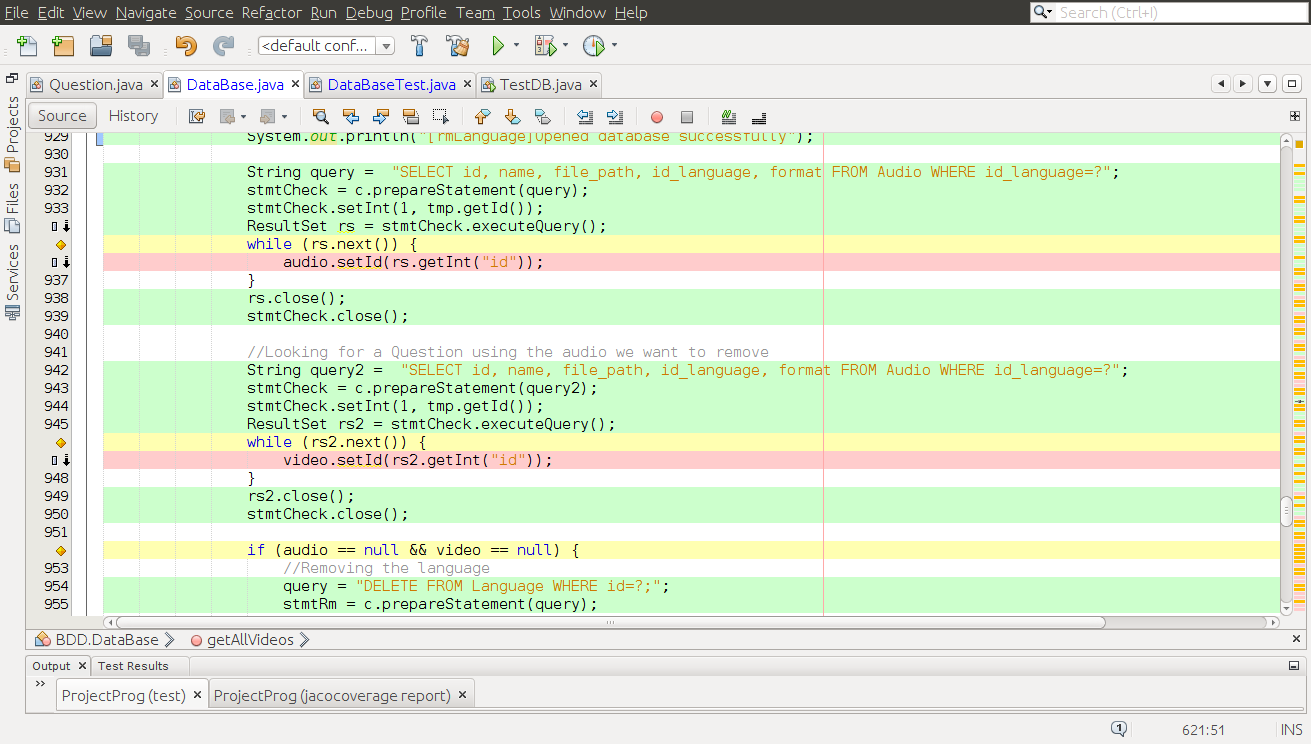
\includegraphics[width=15cm]{./fonctionnement_tests/CoCoJava.png}}
  \caption{Tests - Recouvrement des tests}
  \label{cocojava} 
\end{center}
\end{figure}


\subsection{Performances}

Afin de réaliser les tests de performance, nous avons simplement utilisé un plugin de \textit{Netbeans} (\textsc{Figure} \ref{perf}). Ce plugin permet de mesurer les performance en temps CPU.

Sachant déjà que nous avions un problème de performance pendant le chargement de la page \textit{TestGUI} (voir \ref{GUI}), ce test nous a permis d'identifier le code fautif.
Ainsi, l'accès à la base de données a été mis en cause. La méthode de connexion étant seulement gérée par le driver \textit{SQLite-jdbc}, nous pouvons nous affranchir de tout problème de lenteur dans notre code actuel. Cependant, ce point permet d'envisager une future amélioration à ce niveau là, en déployant un SGBDR plus efficace pour notre utilisation.

\begin{figure}[!ht]
\begin{center}
  \fbox{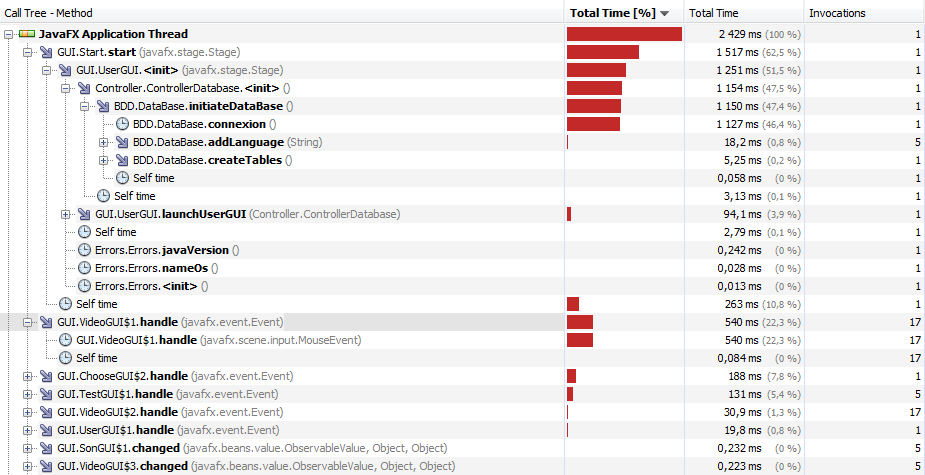
\includegraphics[width=15cm]{./fonctionnement_tests/performance.png}}
  \caption{Tests - Performances}
  \label{perf} 
\end{center}
\end{figure}








\chapter{Bilan}


L'UE de projet de programmation a été important lors de cette première année de master. En effet, elle nous a donné la possibilité de mettre en application les connaissances accumulées durant nos années d'études précédente dans l'élaboration d'un projet. Cependant l'étude de l'existant ainsi que la documentation ont été des parties nouvelles pour nous tous.

Ce projet nous permet d'avoir une ligne supplémentaire dans nos CV respectifs. Plus qu'une mise en situation, c'est, en soit, une expérience professionnelle, puisque nous avions un client à satisfaire.

On peut aussi souligner l'expérience de travail en équipe, qui induit une bonne répartition des tâches, ainsi que l'utilisation d'une gestionnaire de version (dans notre cas, \textit{Github}).

Cependant, notre application n'est pas optimale et plusieurs poursuites de projet peuvent être envisagées :

\begin{itemize}
 \item La sauvegarde et la reprise des test en cas de crash de l'application serait une poursuite à mettre en place dans l'avenir. En effet, notre application extrait les données utilisateur ainsi que ses réponses en fin de test. Malheureusement à cause de ce système, un crash ne permet pas d'avoir une sauvegarde préalable. La solution serait d'écrire dans le fichier texte à chaque validation de réponses. Ensuite en cas d'arrêt non voulu de l'application, un algorithme serait mis en place à partir du fichier créer qui permettrait de retrouver le nombre de question restante.
 \item 
\end{itemize}


L'ajout de la synchronisation audio-vidéo : nos recherches nous ont mené sur deux pistes différentes. La première était l'utilisation de la bibliothèque Xuggle\footnote{http://www.xuggle.com/xuggler/}. Elle utilise les bibliothèques FFmpeg permettant d'encoder, de décoder des fichiers audio et vidéo.
Son utilisation est cependant inappropriée du fait que le projet ait été abandonné et rendant par la même occasion la synchronisation mal venue. En effet aucun support n'est disponible via cette bibliothèque si besoin est.

Par la suite nos recherches nous ont amené à étudier la bibliothèque \textit{Opencv}\footnote{http://opencv.org/}. Elle est la référence dans le domaine du traitement d'images.

Comprenant de nombreuses fonctionnalités, elle possède celles que nous recherchions, c'est à dire la lecture, l'écriture et l'affichage d’une vidéo. Elle nous permettrait notamment la modification du nombre d'images par seconde de notre fichier vidéo pour pouvoir avoir une bonne synchronisation, en prenant pour référence notre fichier audio, et idéalement, les séquences correspondantes de phonèmes.

Nous avons pensé à un algorithme pour pouvoir mixer les deux fichiers. Il a été pensé sur papier mais n'a pas été mis en œuvre, par manque de temps.

\begin{verbnobox}[\small]

Fonction Synchronisation(chemin video, chemin audio):

Vérification lecture et ouverture fichier Video;
Vérification lecture et ouverture  fichier Audio;

Création du fichier de sortie mix;
Récupération des Streams des fichiers audio et video;
Récupération de la StreamAudio pour le fichier audio et récuperation de la Stream Video pour le fichier vidéo;

Si temps_StreamAudio < temps_streamVideo alors
  On augmente frame_rate_StreamVideo jusqu'à temps_StreamAudio = temps_streamVideo;
FinSi;

Si temps_StreamAudio > temps_streamVideo alors
  On diminue le  frame_rate_StreamVideo jusqu'à temps_StreamAudio = temps_streamVideo;
FinSi

Ajout des streams Selectionnées dans le fichier de sortie

Vérification des Streams Selectionnées

Si aucune erreur alors 

  Tant qu'il reste des datas à lire dans le Stream Video ou dans le streamAudio

    Si les datas appartiennent au fichier Video alors
      Tant qu'une image n'est pas complète
	On additionne les packets;
      FinTantQue;
      Si complète alors
	On ajoute l'image à notre fichier de sortie;
      FinSi;
    FinSi;


    Si les datas appartiennent au fichier Audio alors
      Tant qu'un échantillon de la piste audio n'est pas complet
	On additionne les packets;
      FinTantQue;
      Si complet alors
	On ajoute l'image à notre fichier de sortie;
      FinSi;
    FinSi;
    
  FinTantQue;
  
FinSi;

\end{verbnobox}

\textbf{Stream} : un ensemble de données accessible dans le temps. Les éléments d'un stream sont appelés \textit{Frame} et chaque \textit{Frame} est encodé par une sorte différente de codec.


\textbf{Packet} : partition de donnée qui contient des bits. Ces bits sont décodés dans des \textit{Frames} pour que finalement nous puissions les manipuler.




\newpage

%récupérer les citation avec "/footnotemark"
\nocite{*}

%choix du style de la biblio
\bibliographystyle{plain}
%inclusion de la biblio
\bibliography{bibliographie.bib}

\end{document}